\documentclass[10pt,twocolumn]{article}
\usepackage[letterpaper,top=0.75in,bottom=1in,left=0.625in,right=0.625in,columnsep=0.25in]{geometry}
\usepackage{times}\usepackage{mathptmx}
\usepackage[T1]{fontenc}\usepackage[utf8]{inputenc}
\usepackage{amsmath,amssymb,graphicx,booktabs,array,cite,url,microtype,caption,titlesec,float}
\usepackage[hidelinks]{hyperref}
\captionsetup{font=footnotesize,labelfont=footnotesize,labelsep=period,skip=3pt}
\captionsetup[table]{labelfont=footnotesize,textfont=sc,labelformat=simple,labelsep=newline,justification=centering}
\renewcommand{\thetable}{\Roman{table}}
\titleformat{\section}{\centering\normalfont\footnotesize\scshape}{\thesection.}{0.5em}{}
\titleformat{\subsection}{\normalfont\footnotesize\itshape}{\thesubsection)}{0.5em}{}
\renewcommand{\thesection}{\Roman{section}}
\renewcommand{\thesubsection}{\Alph{subsection}}
\titlespacing*{\section}{0pt}{8pt}{4pt}\titlespacing*{\subsection}{0pt}{5pt}{2pt}
\setlength{\parindent}{10pt}\setlength{\parskip}{0pt}
\renewcommand{\arraystretch}{1.08}
\setlength{\textfloatsep}{8pt plus 2pt minus 2pt}\setlength{\floatsep}{6pt plus 2pt minus 2pt}\setlength{\intextsep}{6pt plus 2pt minus 2pt}
\pagestyle{plain}
\begin{document}
\twocolumn[
\begin{center}
{\LARGE\bfseries Pre-training a Character-Level GPT on TinyStories\\[2pt] under a Fixed Compute Budget\par}
\vspace{8pt}
{\large Manidip Debnath\par}
{\small\itshape Oakland University, Rochester, Michigan, USA\par}
{\small manidipdeb@oakland.edu\par}
\vspace{10pt}
\end{center}
\begin{center}\begin{minipage}{0.93\textwidth}
\small\noindent\textbf{\textit{Abstract}---}We implement a nanoGPT-style decoder-only transformer from scratch (0.82\,M parameters, 4 layers, width 128, one token per character) and pre-train it on 40\,M characters of TinyStories. The default configuration reaches a validation loss of 0.857 nats/char (perplexity 2.36, 1.24 bits/char), well below the 1.00 requirement. We then ask how far the loss can be pushed when every training run may use at most $2\times10^{14}$ FLOPs. A two-stage search (12\%-budget screening followed by six full-budget runs and fresh-seed replication) selects a context of 256 characters with batch size 8, which reaches \textbf{0.7016} nats/char (1.012 bits/char, perplexity 2.02) against 0.7513 for the baseline, and stays below 0.725 on all three seeds (mean $0.7060\pm0.0038$). Short-run screening ranked the winning context length last, so short-run rankings did not transfer to the full budget. Part of the gain from a longer context is an artefact of how the fixed-slice evaluation averages over windows, which we state explicitly. As a bonus, replacing learned position embeddings with rotary embeddings (RoPE) lowers the loss at 35\% of the budget in all three seeds (mean gap 0.0087, Welch $p\approx0.04$).
\end{minipage}\end{center}
\begin{center}\begin{minipage}{0.93\textwidth}\small\noindent\textbf{\textit{Index Terms}---}language model, transformer, GPT, TinyStories, character-level tokenization, compute-constrained training, rotary position embedding.\end{minipage}\end{center}
\vspace{6pt}]

\section{Introduction}
Generative pre-trained transformers (GPT) learn to predict the next token of a text and, with scale, acquire fluent language ability \cite{radford2019,vaswani2017}. Small models trained on simple text are a convenient laboratory: TinyStories \cite{eldan2023} shows that children's-story text with a limited vocabulary lets models below one million parameters write coherent stories. This work follows the nanoGPT recipe \cite{karpathy2022} and has three goals: (i)~build every component of a GPT (tokenizer, causal attention, MLP, block, full model, training step) and verify it with unit tests; (ii)~train a default model to a validation loss of at most 1.00 nats/char; and (iii)~minimise the validation loss under a fixed budget of $C_{\max}=2\times10^{14}$ training FLOPs, using a careful and honest experimental protocol. A rotary-embedding variant is studied as an optional extension.

\section{Data and Tokenization}
The training text is a 40\,MB subset of TinyStories (48,793 stories, 39,963,595 characters); the validation text has 27,629 stories and 22,482,104 characters. Tokenization is character-level: the vocabulary has $|V|=96$ entries (newline plus the 95 printable ASCII characters), so the output layer is tiny (12\,K parameters at $d=128$, against 6.4\,M for a 50,257-token BPE vocabulary). Fig.~\ref{fig:freq} shows the most frequent characters; the space alone accounts for about 19\% of the text.

\begin{figure}[t]\centering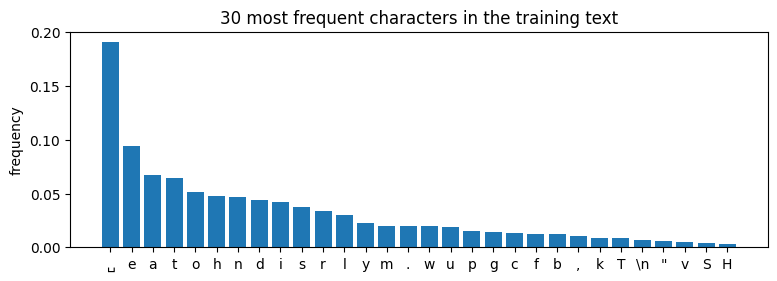
\includegraphics[width=\columnwidth]{figures/cell018.png}
\caption{Thirty most frequent characters of the training text.}\label{fig:freq}\end{figure}

\section{Model Architecture}
The model (Fig.~\ref{fig:arch}) is a pre-norm decoder-only transformer. Token and position embeddings are summed, passed through $n_{\text{layer}}=4$ blocks, a final LayerNorm and a linear head tied to the token embedding.

\begin{figure}[t]\centering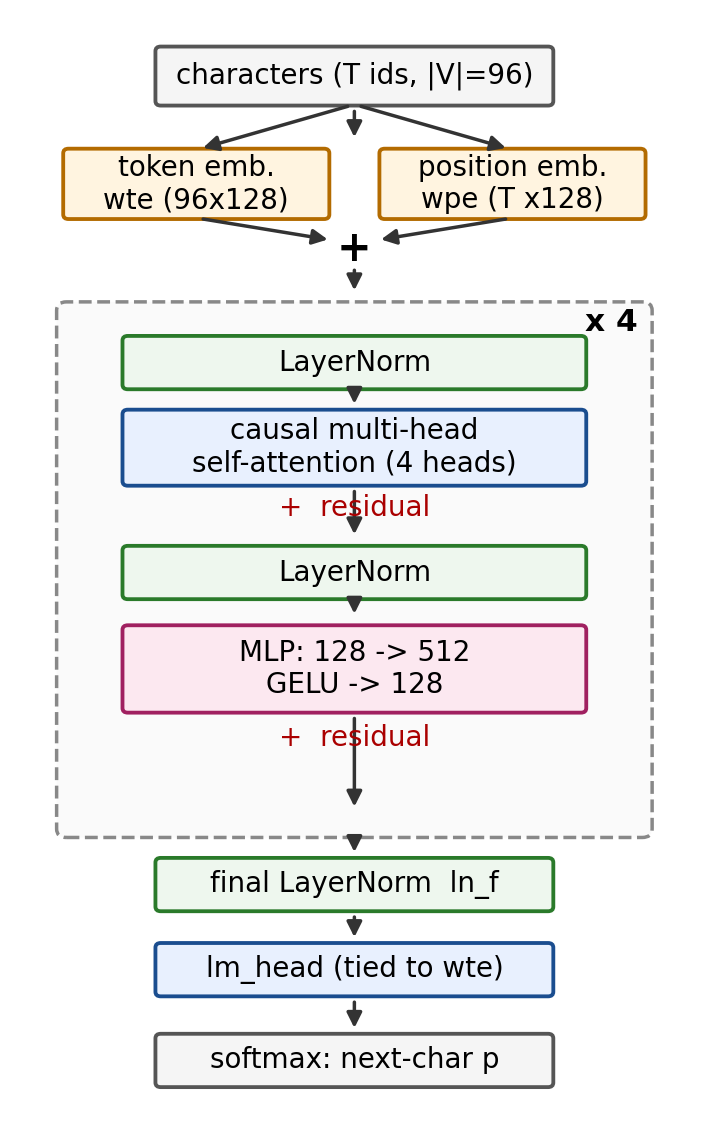
\includegraphics[width=0.62\columnwidth]{figures/fig_architecture.png}
\caption{Architecture of the implemented GPT (default: $d=128$, 4 heads, 4 blocks).}\label{fig:arch}\end{figure}

\subsection{Causal self-attention}
With queries, keys and values $Q,K,V\in\mathbb{R}^{T\times d_k}$ and a causal mask $M$ ($M_{ij}=0$ for $j\le i$, $-\infty$ otherwise),
\begin{equation}
\mathrm{Attn}(Q,K,V)=\mathrm{softmax}\!\Big(\tfrac{QK^{\top}}{\sqrt{d_k}}+M\Big)V .
\end{equation}
Multi-head attention runs $h=4$ heads of width $d_k=d/h=32$ in parallel with one fused projection (\texttt{c\_attn}, width $3d$), concatenates them and applies an output matrix $W_O$. The mask makes future tokens invisible, which a test verifies by changing future inputs and checking that earlier logits do not change.

\subsection{Feed-forward network and block}
The MLP is $\mathrm{MLP}(x)=W_2\,\mathrm{GELU}(W_1x+b_1)+b_2$ with $W_1\in\mathbb{R}^{4d\times d}$. A block applies
\begin{equation}
x\leftarrow x+\mathrm{Attn}(\mathrm{LN}_1(x)),\qquad x\leftarrow x+\mathrm{MLP}(\mathrm{LN}_2(x)).
\end{equation}

\subsection{Parameter count}
The estimate $12d^2$ per block gives $4\cdot12\cdot128^2=786{,}432$ plus embeddings $96\cdot128+128\cdot128=28{,}672$, i.e.\ 815,104. The model has \textbf{822,016} parameters; the difference of 6,912 is exactly the biases and LayerNorm parameters ($1{,}664$ per block $\times4$, plus 256 for the final LayerNorm). The head is tied to the token embedding and adds nothing. Raising the context to 256 adds 128 rows to the position table (+16,384 parameters), giving 838,400.

\section{Training Procedure}
\subsection{Optimisation}
We use AdamW ($\beta=(0.9,0.99)$) \cite{loshchilov2019} with weight decay 0.1 on matrices and embeddings only, gradient clipping at norm 1.0, and a linear warm-up (100 steps) followed by cosine decay from $\eta_{\max}=3\times10^{-3}$ to $\eta_{\min}=3\times10^{-4}$. A training step is: forward pass, clear gradients, backward pass, optimizer update.

\subsection{Compute accounting}
Training compute is estimated as \cite{kaplan2020}
\begin{equation}
C\approx\big(6N+12\,n_{\text{layer}}\,d\,T\big)\times D,\quad D=\text{steps}\times B\times T,
\end{equation}
where $N$ is the parameter count, $B$ the batch size and $T$ the context length. The attention term grows with $T$, so at a fixed $C$ a longer context sees fewer tokens. A budget planner converts a fraction of $C_{\max}$ into a number of steps with exactly this formula, so no run can exceed the budget.

\subsection{Default run}
The default model (3,000 steps, batch 32, $T=128$) uses $7.0\times10^{13}$ FLOPs (35\% of the budget) and trains in 0.8 minutes on a Tesla T4. Training and validation loss fall together from $\ln 96\approx4.56$ (Fig.~\ref{fig:default}); an early smoke test checks that 200 steps already bring the loss below 2.5. Fig.~\ref{fig:lr} (left) illustrates the schedule shape.

\begin{figure}[t]\centering
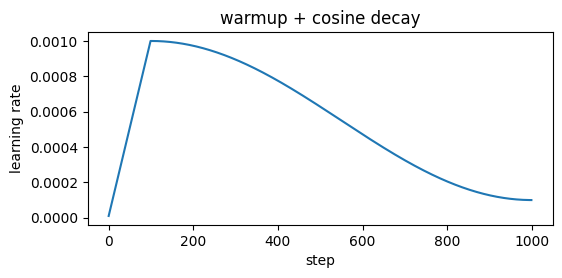
\includegraphics[width=0.49\columnwidth]{figures/cell049.png}\hfill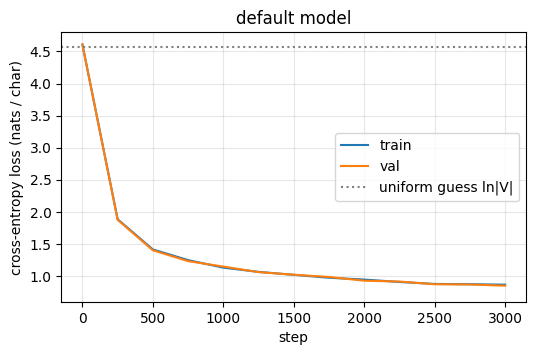
\includegraphics[width=0.49\columnwidth]{figures/cell057.png}
\caption{Left: shape of the warm-up and cosine-decay schedule (unit-test plot with $\eta_{\max}=10^{-3}$, 1,000 steps). Right: training and validation loss of the default model; the dotted line is the uniform guess $\ln|V|$.}\label{fig:default}\label{fig:lr}\end{figure}

\section{Evaluation Protocol}
\subsection{Fixed-slice loss}
The training-time \texttt{estimate\_loss} averages random batches and is noisy (standard error about 0.003--0.004). All comparisons therefore use a deterministic \emph{fixed-slice} loss: the first $10^6$ validation characters are cut into consecutive windows of the model's own \texttt{block\_size}, and the mean cross-entropy over all windows is reported. Part~8 of the assignment uses the same slice.

\subsection{Reference baselines}
Table~\ref{tab:base} gives context-free references computed from training counts, and the default and final models, in three units: nats/char, perplexity $e^{\mathcal L}$ and bits/char $\mathcal L/\ln2$ (compression is relative to 8-bit ASCII).

\begin{table}[t]\centering\caption{Baselines and models on the fixed validation slice}\label{tab:base}
\footnotesize\begin{tabular}{lcccc}\toprule
Model & Loss & Perplexity & bits/char & Compr.\\\midrule
Uniform & 4.5643 & 96.00 & 6.585 & 1.2$\times$\\
Unigram & 3.0806 & 21.77 & 4.444 & 1.8$\times$\\
Bigram & 2.2800 & 9.78 & 3.289 & 2.4$\times$\\
Default GPT (3,000 steps) & 0.8570 & 2.36 & 1.236 & 6.5$\times$\\
\textbf{Final GPT (full budget)} & \textbf{0.7016} & \textbf{2.02} & \textbf{1.012} & \textbf{7.9}$\times$\\\bottomrule\end{tabular}\end{table}

\section{Experiments Under the Compute Budget}
\subsection{Search protocol}
Fig.~\ref{fig:flow} summarises the protocol. The rule for choosing the final model was fixed before the runs: take the setting with the lowest fixed-slice loss at the full budget (seed 1337), then replicate the winner and the baseline with two fresh seeds, because selecting on one seed is biased in favour of the winner. All Part~7 models are the assignment's \texttt{GPT} trained with \texttt{train()}; only the knobs context length, batch size and learning rate are changed, and every run uses at most $0.995\,C_{\max}$.

\begin{figure*}[t]\centering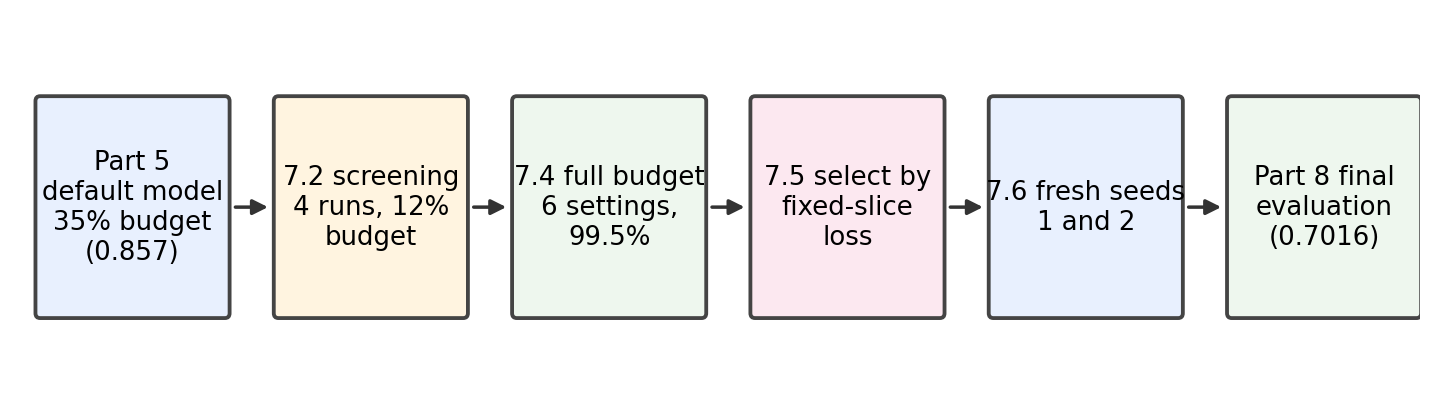
\includegraphics[width=0.85\textwidth]{figures/fig_workflow.png}\caption{Experimental workflow of Part~7.}\label{fig:flow}\end{figure*}

\subsection{Screening at 12\% of the budget}
Four candidates were trained for 12\% of the budget (Table~\ref{tab:screen}, Fig.~\ref{fig:screen}). A candidate had to beat the baseline by a margin of 0.010 to be chosen in advance; none did (best: weight decay 0.01, $-0.0055$), so screening alone would have kept the baseline. The context-256 candidate ranked \emph{last} (+0.1716).

\begin{table}[t]\centering\caption{Screening runs (12\% budget, fixed-slice loss)}\label{tab:screen}
\footnotesize\begin{tabular}{lcc}\toprule
Candidate & Loss & vs.\ base\\\midrule
wd 0.01 & 1.0961 & $-0.0055$\\
base ($\eta=3\mathrm{e}{-3}$) & 1.1015 & 0\\
$\eta=2\mathrm{e}{-3}$ & 1.1524 & $+0.0509$\\
context 256 (batch 16) & 1.2731 & $+0.1716$\\\bottomrule\end{tabular}\end{table}

\begin{figure}[t]\centering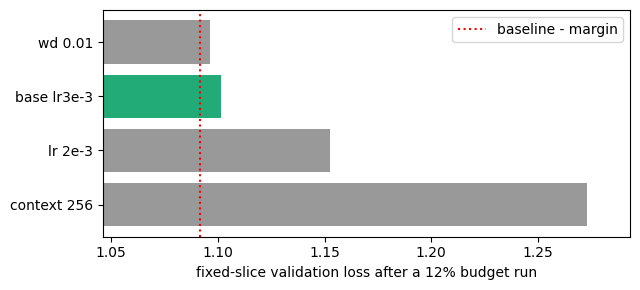
\includegraphics[width=0.92\columnwidth]{figures/cell079.png}\caption{Screening result. The red line is the baseline minus the 0.010 margin.}\label{fig:screen}\end{figure}

\subsection{Full-budget runs}
Because short runs can mislead, six settings were then trained with 99.5\% of the budget (about 2.4--2.9 minutes each on a T4). Table~\ref{tab:full} gives the result and Fig.~\ref{fig:curves} the learning curves.

\begin{table}[t]\centering\caption{Full-budget runs (seed 1337, fixed-slice loss)}\label{tab:full}
\footnotesize\begin{tabular}{lrrcr}\toprule
Setting & Params & Steps & Loss & $\Delta$\\\midrule
\textbf{T256, batch 8} & 838,400 & 14,715 & \textbf{0.7016} & $-0.0496$\\
T256, batch 16, $\eta{=}4\mathrm{e}{-3}$ & 838,400 & 7,357 & 0.7060 & $-0.0452$\\
T512, batch 8 & 871,168 & 5,802 & 0.7187 & $-0.0326$\\
T384, batch 8 & 854,784 & 8,650 & 0.7211 & $-0.0301$\\
T256, batch 16 & 838,400 & 7,357 & 0.7385 & $-0.0128$\\
T128, batch 32 (baseline) & 822,016 & 8,495 & 0.7513 & 0\\\bottomrule\end{tabular}\end{table}

\begin{figure*}[t]\centering
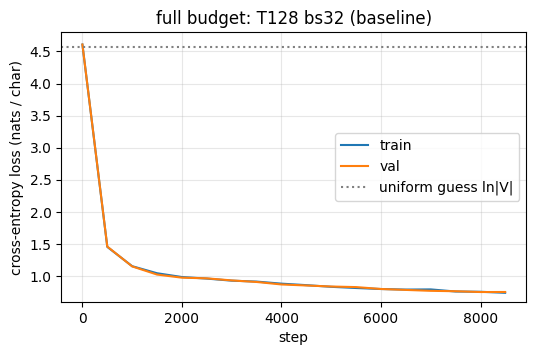
\includegraphics[width=0.32\textwidth]{figures/cell082.png}\hfill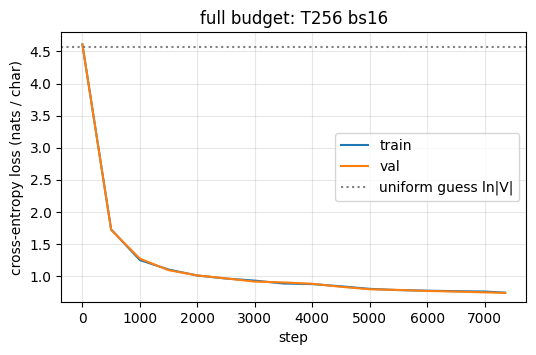
\includegraphics[width=0.32\textwidth]{figures/cell083.png}\hfill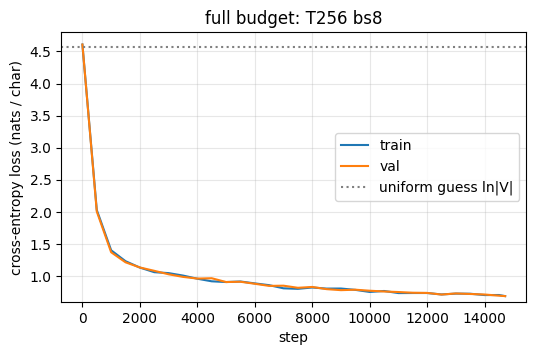
\includegraphics[width=0.32\textwidth]{figures/cell084.png}\\[3pt]
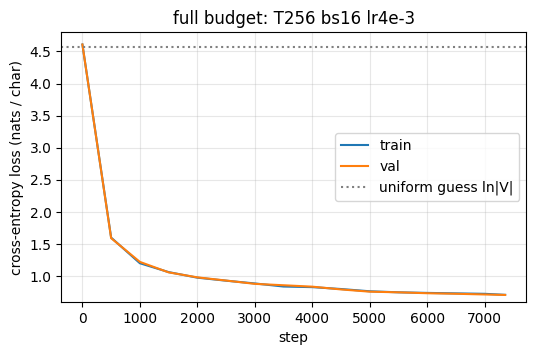
\includegraphics[width=0.32\textwidth]{figures/cell085.png}\hfill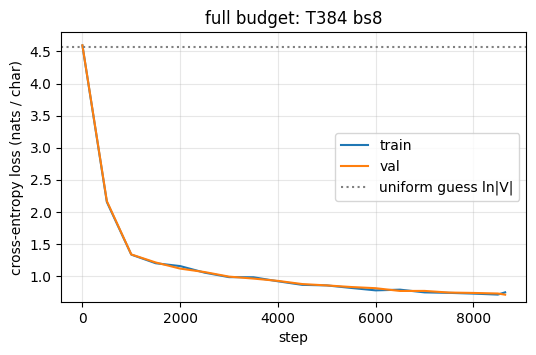
\includegraphics[width=0.32\textwidth]{figures/cell086.png}\hfill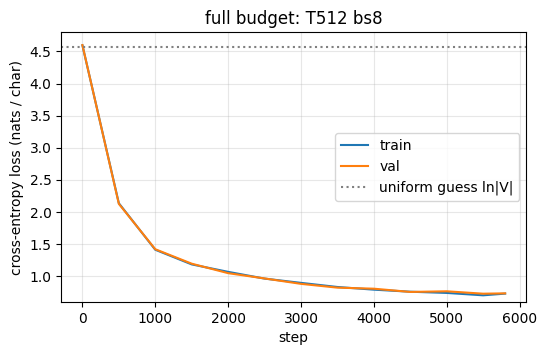
\includegraphics[width=0.32\textwidth]{figures/cell087.png}
\caption{Training and validation loss of the six full-budget runs (top: T128 bs32 baseline, T256 bs16, T256 bs8; bottom: T256 bs16 $\eta{=}4\mathrm{e}{-3}$, T384 bs8, T512 bs8).}\label{fig:curves}\end{figure*}

Three observations follow. (1)~Moving from context 128 to 256 at equal tokens per step (batch 16) lowers the loss by 0.0128. (2)~Halving the batch to 8 doubles the number of updates and lowers it by a further 0.0369; a higher learning rate at batch 16 gives most of the same gain (0.7060). `T256 bs8' sees fewer characters than the baseline (30.1\,M against 34.8\,M) but performs 1.7 times as many updates, so at this budget the model is limited by the number of updates and not by the amount of text. (3)~Contexts longer than 256 did not pay off: the attention term makes tokens more expensive, so only 8,650 (T384) and 5,802 (T512) steps fit. Overall the run table and the compute plot are shown in Fig.~\ref{fig:compute}.

\begin{figure*}[t]\centering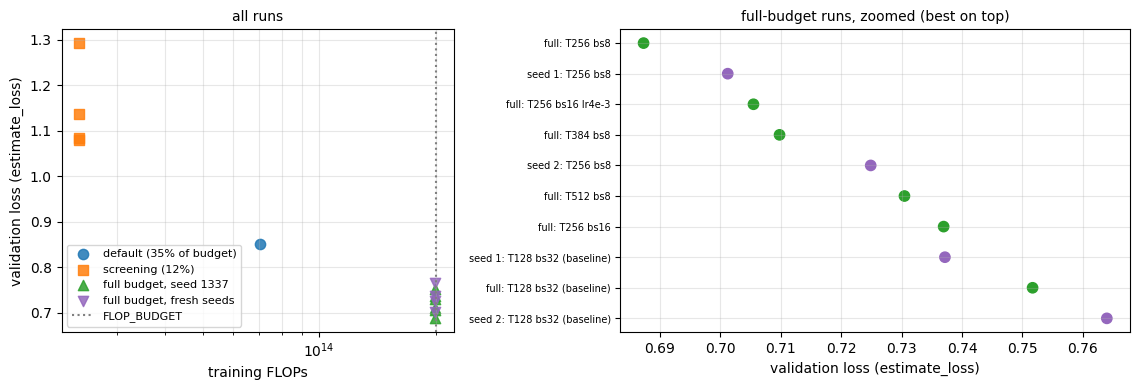
\includegraphics[width=0.9\textwidth]{figures/cell099.png}\caption{Validation loss (from \texttt{estimate\_loss}) against training FLOPs for every run. Left: all runs; right: the nine full-budget runs ranked, best on top (green: seed 1337, purple: fresh seeds).}\label{fig:compute}\end{figure*}

\subsection{Fresh seeds}
Table~\ref{tab:seed} replicates the baseline and the winner with seeds 1 and 2. On the two fresh seeds the baseline averages 0.7560 and the winner 0.7082, a gain of 0.0477, more than 12 times the larger seed standard deviation (0.0038). All three seeds of the winner are below the 0.725 threshold (worst 0.7088, margin 0.016), so the tier does not depend on the seed. The winner was chosen among six settings on the same slice it is scored on, which favours it slightly; this is why the fresh seeds are reported.

\begin{table}[t]\centering\caption{Seed replication (fixed-slice loss)}\label{tab:seed}
\footnotesize\begin{tabular}{lccccc}\toprule
Setting & 1337 & 1 & 2 & Mean & Std\\\midrule
T128 bs32 & 0.7513 & 0.7564 & 0.7555 & 0.7544 & 0.0027\\
T256 bs8 & 0.7016 & 0.7077 & 0.7088 & 0.7060 & 0.0038\\\bottomrule\end{tabular}\end{table}

\subsection{Loss by position and the scoring artefact}
Fig.~\ref{fig:pos} plots the loss against the position inside the window. At position 0 the model has seen one character and its loss (about 2.3) is close to the bigram baseline (2.28); after about ten characters it is near 1.0, and it keeps falling slowly. The final model (context 256) lies below the default one at almost every position. Because the evaluation averages over whole windows of the model's own length, a longer window contains a smaller share of the expensive first characters, which lowers the \emph{measured} loss by itself. Part of the 128$\to$256 gain is therefore a property of the scoring and not of a better language model; we did not quantify how much. We also did not test the baseline context (128) with batch 8, so the gain cannot be split cleanly between context and smaller batch.

\begin{figure}[t]\centering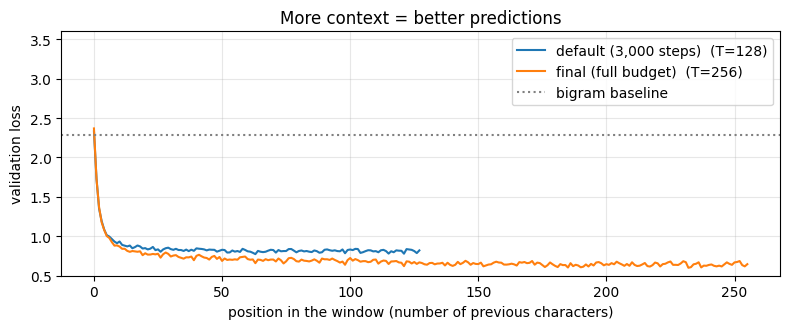
\includegraphics[width=\columnwidth]{figures/cell108.png}\caption{Fixed-slice loss by position in the window for the default (T=128) and final (T=256) models.}\label{fig:pos}\end{figure}

\subsection{Samples and temperature}
Generation divides the logits by a temperature $\tau$: $p_i=e^{z_i/\tau}/\sum_je^{z_j/\tau}$. At $\tau=0.5$ the distribution is sharpened: every word is real and the sentences are short and grammatical, but phrases repeat (``a big tree'', ``a big seek'', ``a big dream''). At $\tau=1.0$ names and sentence shapes are plausible but spelling and grammar errors appear (``boury'', ``weater''). At $\tau=1.5$ the distribution is flat and errors compound, producing non-words (``broes'', ``vehion'') and misplaced punctuation. A vocabulary check shows that 99.1\% of the 845 words generated by the final model at $\tau=0.8$ occur at least three times in the training text, against 98.5\% of 826 for the default model; this difference is not significant (one standard error of a rate near 99\% is 0.4--0.5 points), and the metric cannot measure coherence. As expected for a base model, it \emph{continues} text instead of answering: after ``The capital of France is'' it writes story fragments, because its only training objective is next-character prediction on stories.

\section{Bonus: Rotary Position Embeddings}
Rotary embeddings (RoPE) \cite{su2021} remove the learned position table. Each head's query and key are rotated by position-dependent angles before the scores are computed, so $\langle R_iq,R_jk\rangle$ depends only on $i-j$; the value vector is left unchanged. The RoPE model has 805,632 parameters (16,384 fewer, exactly the removed table). Four tests pass: position 0 is not rotated, rotations preserve vector length, scores are unchanged when both positions shift by the same amount, and attention remains causal.

At the default setting (35\% of the budget, same configuration, learning rate, seed and data), RoPE reaches a fixed-slice loss of 0.8437 against 0.8570 for learned positions (paired difference $0.0134\pm0.0005$ over 7,812 windows, RoPE better on 61.9\%). Its validation loss is lower at every logged step, most strongly early (1.41 against 1.88 at step 250; Fig.~\ref{fig:rope}).

\begin{figure*}[t]\centering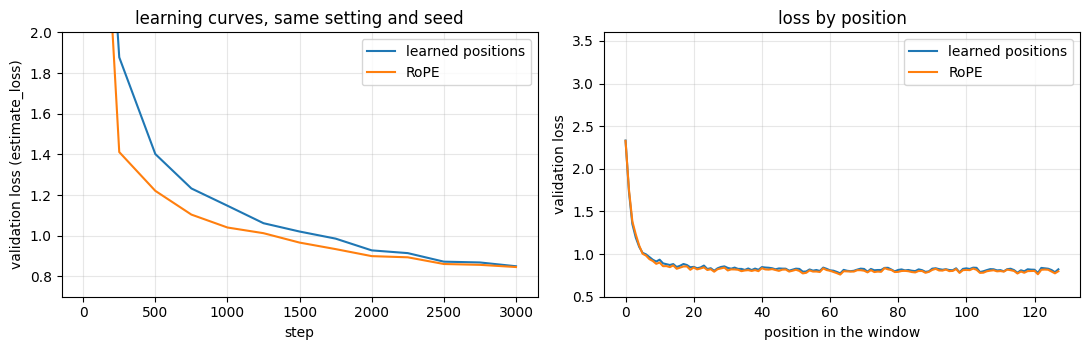
\includegraphics[width=0.9\textwidth]{figures/cell125.png}\caption{RoPE against learned positions at the default setting. Left: learning curves; right: loss by position.}\label{fig:rope}\end{figure*}

A seed replication (Table~\ref{tab:rope}, Fig.~\ref{fig:ropeseeds}) gives $0.8473\pm0.0036$ for RoPE against $0.8561\pm0.0015$ for learned positions; the mean gap of 0.0087 is 3.8 standard errors of the seed spread, and every RoPE seed is below every learned-position seed (probability 1/20 if the runs were exchangeable). A Welch $t$-test gives $p\approx0.04$, so the evidence is moderate, not conclusive. Limits: all RoPE results are at 35\% of the budget; there are three seeds per model; and the RoPE model is not the Part~7 model, since the final model must come from \texttt{train()}, which builds the original \texttt{GPT}.

\begin{table}[t]\centering\caption{RoPE against learned positions (35\% budget)}\label{tab:rope}
\footnotesize\begin{tabular}{lccccc}\toprule
Model & 1337 & 1 & 2 & Mean & Std\\\midrule
Learned & 0.8570 & 0.8567 & 0.8544 & 0.8561 & 0.0015\\
RoPE & 0.8437 & 0.8473 & 0.8510 & 0.8473 & 0.0036\\\bottomrule\end{tabular}\end{table}

\begin{figure}[t]\centering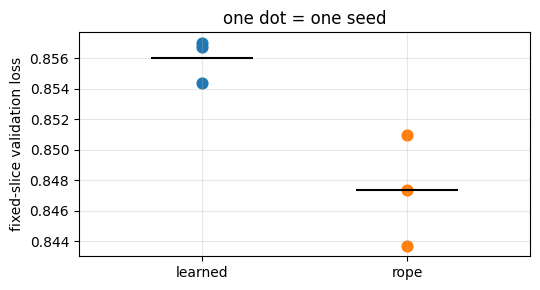
\includegraphics[width=0.8\columnwidth]{figures/cell135.png}\caption{One dot per seed; black bars are means.}\label{fig:ropeseeds}\end{figure}

\section{Discussion and Limitations}
Compute mattered most: using the full budget instead of 35\% lowers the baseline from 0.8570 to 0.7513. At a fixed budget the best use was a longer context with a smaller batch, which buys more optimizer updates. Short-run (12\%) rankings failed to predict this, so comparisons were made at the full budget. No overfitting occurs: the final run processes 30.1\,M characters, 0.75 of one pass over the 40\,M training characters, and training and validation loss are equal at the last step (0.688 and 0.687). Limitations: one hardware type (T4, GPU runs are not bit-for-bit reproducible, so a re-run changes the last digits); selection on a single slice; the position-averaging artefact described above; model width and depth at long context and RoPE at the full budget were not tested.

\section{Conclusion}
A from-scratch character-level GPT with 0.82\,M parameters reaches 0.857 nats/char with the default setting and \textbf{0.7016} nats/char (perplexity 2.02, 1.01 bits/char, 7.9$\times$ compression) under a $2\times10^{14}$-FLOP budget, with context 256 and batch 8. The gain over the baseline is 12 times larger than the seed noise. Rotary embeddings give a further moderate improvement at 35\% of the budget.

\section*{Acknowledgment}
This report accompanies the notebook \texttt{nanogpt\_pretraining\_final\_Manidip\_Debnath\_v4.ipynb}; all numbers are taken from its executed outputs (one run on a Google Colab Tesla T4).

\begin{thebibliography}{9}\footnotesize
\bibitem{vaswani2017}A.~Vaswani \emph{et al.}, ``Attention is all you need,'' in \emph{Proc.\ NeurIPS}, 2017.
\bibitem{radford2019}A.~Radford \emph{et al.}, ``Language models are unsupervised multitask learners,'' OpenAI, 2019.
\bibitem{karpathy2022}A.~Karpathy, ``nanoGPT,'' 2022. [Online]. Available: \url{https://github.com/karpathy/nanoGPT}
\bibitem{eldan2023}R.~Eldan and Y.~Li, ``TinyStories: How small can language models be and still speak coherent English?'' arXiv:2305.07759, 2023.
\bibitem{kaplan2020}J.~Kaplan \emph{et al.}, ``Scaling laws for neural language models,'' arXiv:2001.08361, 2020.
\bibitem{su2021}J.~Su \emph{et al.}, ``RoFormer: Enhanced transformer with rotary position embedding,'' arXiv:2104.09864, 2021.
\bibitem{loshchilov2019}I.~Loshchilov and F.~Hutter, ``Decoupled weight decay regularization,'' in \emph{Proc.\ ICLR}, 2019.
\end{thebibliography}
\end{document}
